% !TeX root = RJwrapper.tex
\title{A clustering algorithm to organize satellite hotspots data for the
purpose of tracking bushfires remotely}
\author{by Weihao Li, Emily Dodwell, and Dianne Cook}

\maketitle

\abstract{%
An abstract of less than 150 words.
}

\hypertarget{introduction}{%
\subsection{Introduction}\label{introduction}}

Bushfires are a major problem for Australia, and many other parts of the
globe. There is concern that as the climate becomes hotter, and drier,
that the impact of fires becomes much more severe and extensive. In
Australia, the 2019-2020 fires were the worst on record causing
extensive ecological damage, as well as damage to agricultural
resources, properties and infrastructure. The Wollemi pine, rare
prehistoric trees, required special forces intervention to prevent the
last stands in the world, in remote wilderness areas, from being turned
into ash.

Contributing to the problem is that many fires started in very remote
areas, locations deep into the temperate forests ignited by lightning,
that are virtually impossible to access or to monitor. Satellite data
provides a possible solution to this, particularly remotely sensed
hotspot data, which may be useful in detecting new ignitions and
movements of fires. Understanding fires in remote areas using satellite
data may provide some help in developing effective strategies for
mitigating bushfire impact.

This work addresses this topic. Using hotspot data, can we cluster in
space and time, in order to determine (1) points of ignition and (2)
track the movement of bushfires.

This paper is organised as follows. The next section provides an
introduction to the literature on spatiotemporal clustering and bushfire
modeling and dynamics. Section \protect\hyperlink{algorithm}{Algorithm}
describes the clustering algorithm, and section
\protect\hyperlink{application}{Application} illustrates how the
resulting data can be used to study bushfire ignition.

\hypertarget{background}{%
\subsection{Background}\label{background}}

literature review

\hypertarget{algorithm}{%
\subsection{Algorithm}\label{algorithm}}

\hypertarget{data-source}{%
\subsubsection{Data source}\label{data-source}}

This algorithm is initially developed in the research of 2019-2020
bushfires in Victoria, Australia. Therefore, the illustration of this
algorithm will use hotspot data during 2019-2020 Australian bushfire
season taken from Himawari-8 satellite \citep{jaxa}. This satellite
hotpot dataset contains records of 1989572 hotspots for 6 months in the
full disk of 140 \textdegree east longitude.

The data pre-processing procedure includes selecting hotspots within the
boundary of Victoria and filtering hotspots with a threshold (irradiance
over 100 watts per square metre) suggested by \citet{hotspots} to reduce
noise from the background.

The final dataset contains 75936 hotspots with ID, longitude, latitude
and observed date as fields. The map of this dataset is shown in Figure
\ref{fig:hotspots}.

\begin{Schunk}
\begin{figure}

{\centering 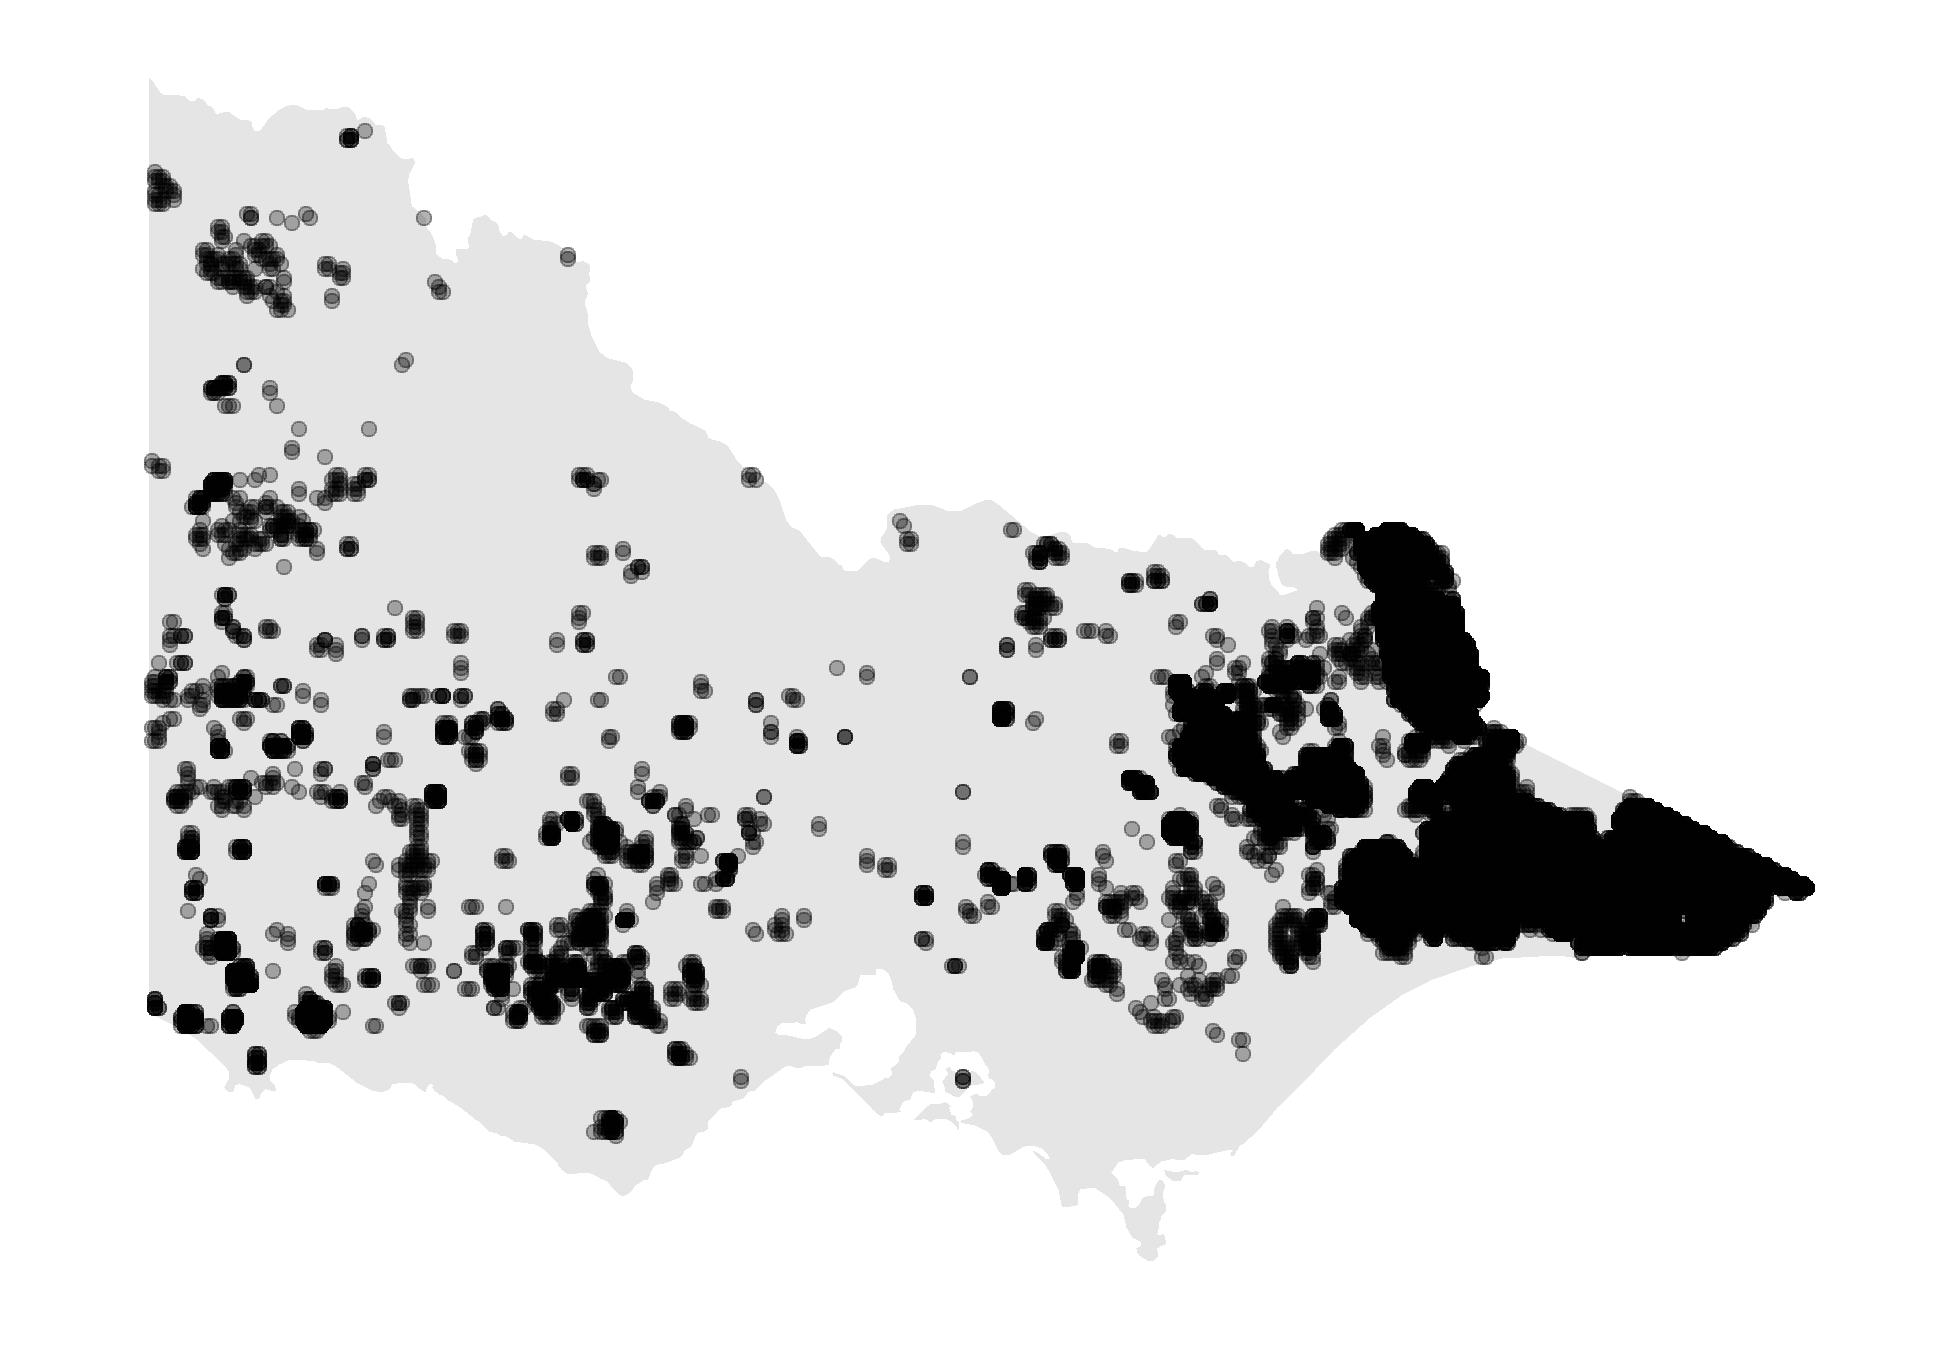
\includegraphics[width=0.8\linewidth]{figures/before_clustering} 

}

\caption[A map shows the distribution of hotspots in Victoria during 2019-2020 Australia bushfire season]{A map shows the distribution of hotspots in Victoria during 2019-2020 Australia bushfire season.}\label{fig:hotspots}
\end{figure}
\end{Schunk}

\hypertarget{steps}{%
\subsubsection{Steps}\label{steps}}

The spatiotemporal clustering algorithm is consist of 4 steps, (1)
divide hotspots into intervals, (2) cluster hotspots spatially, (3)
update the memberships and (4) compute ignition locations. They will be
described in details in the rest of the section.

\textbf{1. Divide hotspots into intervals}

Despite hotspot data can be represented in the three-dimensional
Euclidean space and clustered using ordinary algorithms, like K-means,
the clustering results could be highly sensitive to the scaling of the
temporal dimension \citep{kisilevich2009spatio}. Besides, one of the
characteristics of the hotspot data is cloud cover could lead to missing
observations of a bushfire in several hours. It suggests that hotspots
with long intervals may belong to the same bushfire. One possible
solution to this issue is dividing hotspot data into intervals. In other
words, the temporal dependence between hotspots is predetermined by a
parameter \(ActiveTime\). The interpretation of \(ActiveTime\) is the
time a fire can stay smouldering but undetectable by satellite before
flaring up again.

Given a certain value of \(ActiveTime\) and the length of the time frame
\(T\), the algorithm will define several intervals,

\[\boldsymbol{S}_t = [max(1,t-ActiveTime),t],~~t = 1,2,...,T\]

,where \(T\) and \(t\) have the same unit as \(ActiveTime\).

For example, if the dataset contains 48 hours of hotspot data and the
\(ACtiveTime = 24~hours\), there will be 48 intervals,
\(\boldsymbol{S}_1,\boldsymbol{S}_2,..,\boldsymbol{S}_{48}\), where

\begin{align*}
\boldsymbol{S}_1 &= [1,1]\\
\boldsymbol{S}_2 &= [1,2]\\
&...\\
\boldsymbol{S}_{25} &= [1,25]\\
\boldsymbol{S}_{26} &= [2,26]\\
&...\\
\boldsymbol{S}_{47} &= [23,47]\\
\boldsymbol{S}_{48} &= [24,48]
\end{align*}

\textbf{2. Cluster hotspots spatially}

The previous step breaks the temporal dimension. Hence, the following
step only needs to address the hotspots spatially by introducing another
parameter \(AdjDist\). \(AdjDist\) represents the potential distance a
fire can spread with respect to the temporal resolution of the data. For
example, let \(AdjDist = 3000 m\) and the temporal resolution of the
data is 10-minute, then the potential speed of the bushfire is
\(3000m/10~min = 18km/h\).

Given a fixed value of \(AdjDist\) and the interval
\(\boldsymbol{S}_t\), the algorithm will:

\begin{enumerate}
\def\labelenumi{(\alph{enumi})}
\item
  Append a randomly selected hotspot \(h_i\) to a empty list
  \(\boldsymbol{L}\), where \(h_i\) is the \(i\)th hotspot in the
  interval \(\boldsymbol{S}_t\), and let pointer \(\boldsymbol{P}\)
  points to the first element of the list \(\boldsymbol{L}\).
\item
  Visit every \(h_i\) where \(h_i \notin \boldsymbol{L}\). If
  \(geodesic(h_i, \boldsymbol{P})\leq AdjDist\), append \(h_i\) to list
  \(\boldsymbol{L}\).
\item
  Move pointer \(\boldsymbol{P}\) to the next item of the list
  \(\boldsymbol{L}\).
\item
  Repeat (b) and (c) till the pointer \(\boldsymbol{P}\) reaches to the
  end of the list \(\boldsymbol{L}\).
\item
  For all hotspots \(h_i \in \boldsymbol{L}\), assign a new membership
  to them. Pop these hotspots from the interval \(\boldsymbol{S}_t\).
  Repeat (a) to (e) if interval \(\boldsymbol{S}_t\) is not empty.
\item
  Recover the interval \(\boldsymbol{S}_t\) and record the memberships.
\end{enumerate}

Diagram \ref{fig:step2figs} shows an example of this step.

\begin{Schunk}
\begin{figure}

{\centering 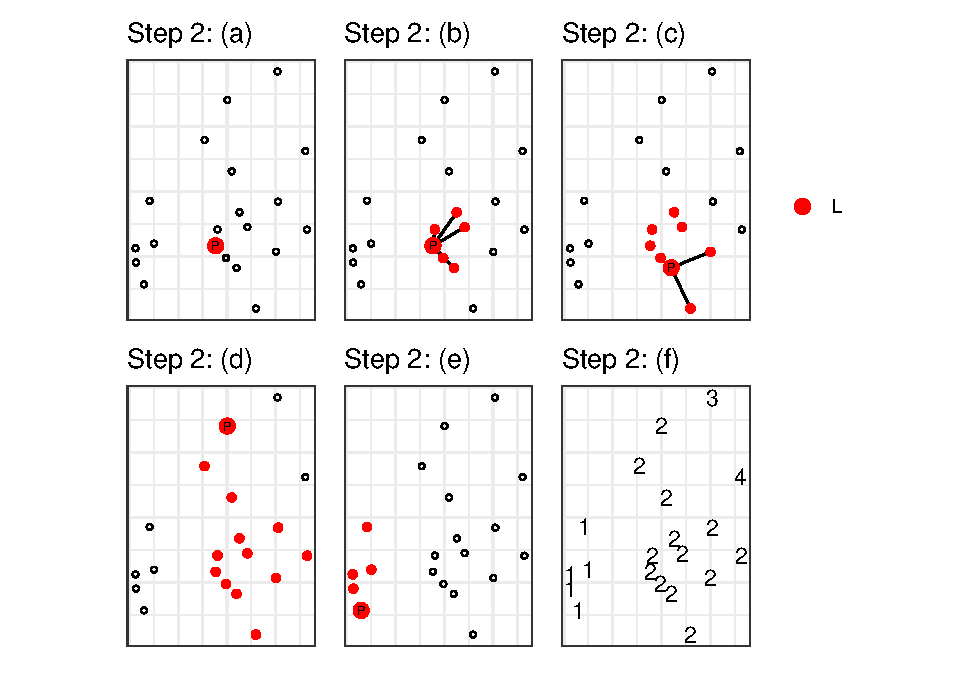
\includegraphics[width=0.8\linewidth]{clustering_paper_files/figure-latex/step2figs-1} 

}

\caption{An example of step 2 given 20 hotspots in interval $\boldsymbol{S}_t$. (a) A hotspot is selected randomly as the first item of list $\boldsymbol{L}$ and the pointer $\boldsymbol{P}$. Hotspots in list $\boldsymbol{L}$ are in red. Pointer $\boldsymbol{P}$ is drawn with larger marker size. (b) Nearby hotspots of the pointer $\boldsymbol{P}$ are appended to the list $\boldsymbol{L}$. (c) Move pointer $\boldsymbol{P}$ to the next item of list $\boldsymbol{L}$ and append the nearby hotspots to list $\boldsymbol{L}$. (d) The first cluster is identified via repeating substep (c). (e) Clear the list $\boldsymbol{L}$, then randomly select an unassigned hotspot to identify another cluster. (f) The final clustering result is produced via repeating substep (d). The labels show the cluster each hotspot belongs to.}\label{fig:step2figs}
\end{figure}
\end{Schunk}

\textbf{3. Update the memberships}

With clustering results for each interval, the next step is to update
the memberships by bringing in information from earlier intervals.

This step starts from \(t=2\) till \(t=T\). Given the interval
\(\boldsymbol{S}_t\), the algorithm will,

\begin{enumerate}
\def\labelenumi{(\alph{enumi})}
\item
  Let \(h_i\) succeeds its membership from \(\boldsymbol{S}_{t-1}\), if
  \(h_i\) belongs to \(\boldsymbol{S}_{t-1}\), where \(h_i\) is the
  \(i\)th hotspot in the interval \(\boldsymbol{S}_t\). These hotspots
  are collected by a set \(\boldsymbol{H}_s = \{h_s^1,h_s^2,...\}\).
\item
  Set \(\boldsymbol{H}_c = \{h_c^1,h_c^2,...\}\), where \(h_c^i\) is the
  \(i\)th hotspot in set \(\boldsymbol{H}_c\). \(h_c^i\) belongs to
  \(\boldsymbol{S}_t\) but does not belong to \(\boldsymbol{S}_{t-1}\).
  If \(h_c^i\) being clustered into the same component with \(h_s^j\) in
  interval \(\boldsymbol{S}_t\), \(h_c^i\) succeeds the membership from
  the nearest \(h_s^j\), where \(h_s^j\) is the \(j\)th hotspot in set
  \(\boldsymbol{H}_s\).
\end{enumerate}

\begin{Schunk}
\begin{figure}

{\centering 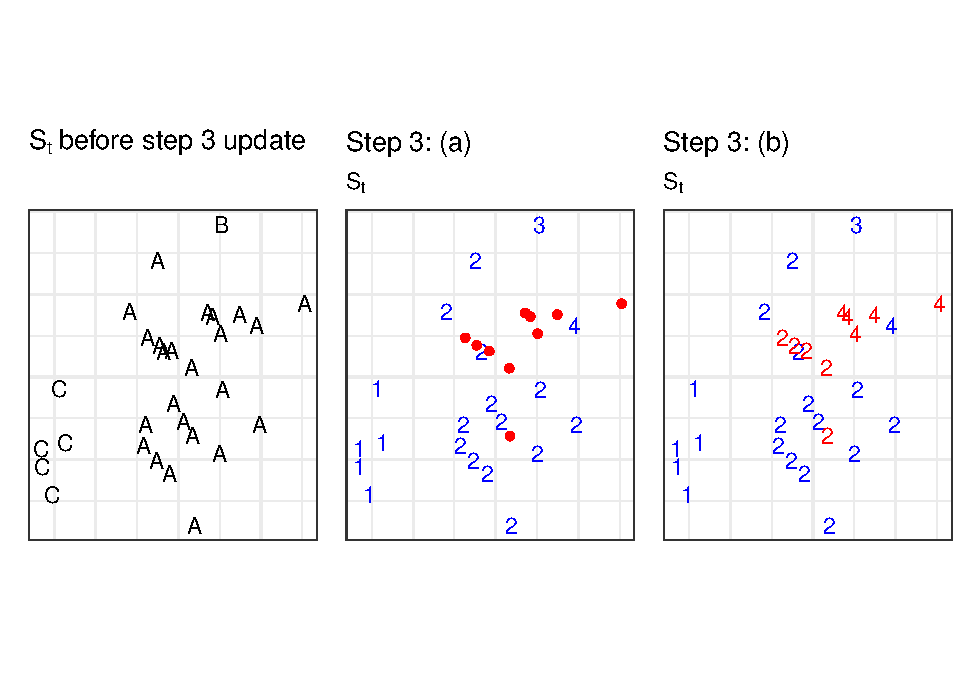
\includegraphics[width=0.8\linewidth]{clustering_paper_files/figure-latex/step3figs-1} 

}

\caption{An example of step 3. In this example, there are 30 hotspots in interval $\boldsymbol{S}_t$ (a) 20 out of 30 hotspots belong to both interval $\boldsymbol{S}_t$ and interval $\boldsymbol{S}_{t-1}$. These hotspots succeed their memberships from $\boldsymbol{S}_{t-1}$. They are annotated in blue with membership labels. Points in red are the rest 10 hotspots that only belong to interval $\boldsymbol{S}_t$. (b) For each red point, succeeds the nearest blue label that shares the same component (according to the left plot) with that red point in interval $\boldsymbol{S}_t$. }\label{fig:step3figs}
\end{figure}
\end{Schunk}

\textbf{4. Compute ignition locations}

The previous step assigns all hotspots with updated memberships. Hence,
the final step is to compute the ignition location for each cluster. If
there are multiple earliest hotspots belong to the same cluster, the
centroid of these hotspots is used as the ignition location. Otherwise,
the earliest hotspot is used as the ignition location.

\hypertarget{effects-of-parameter-choices}{%
\subsubsection{Effects of parameter
choices}\label{effects-of-parameter-choices}}

There are two parameters that can be tuned in this algorithm, which are
\(AdjDist\) and \(ActiveTime\). Increase \(AdjDist\) or the
\(ActiveTime\) will usually reduce the number of clusters. However, if
there are large gaps between clusters spatially and temporally, increase
\(ActiveTime\) and \(AdjDist\) will not significantly reduce the number
of clusters. Given one of the metrics to evaluate the goodness of the
clustering is the gap between clusters, the optimal choice of
\(AdjDist\) and \(ActiveTime\) can be chosen when they have minimum
impact on the number of clusters. However, under this setting, the
optimal \(ActiveTime\) and \(AdjDist\) will approach to infinitely as
the number of clusters approach to 1. Hence, a restriction needs to be
applied on this optimization. Increase of \(ActiveTime\) and \(AdjDist\)
will only be allowed when there is a major fall of the number of
clusters. Due to its similarity to determining the number of principal
components to keep in a principal component analysis, a visualization
tool is developed inspired by the scree plot.

\begin{Schunk}
\begin{figure}

{\centering 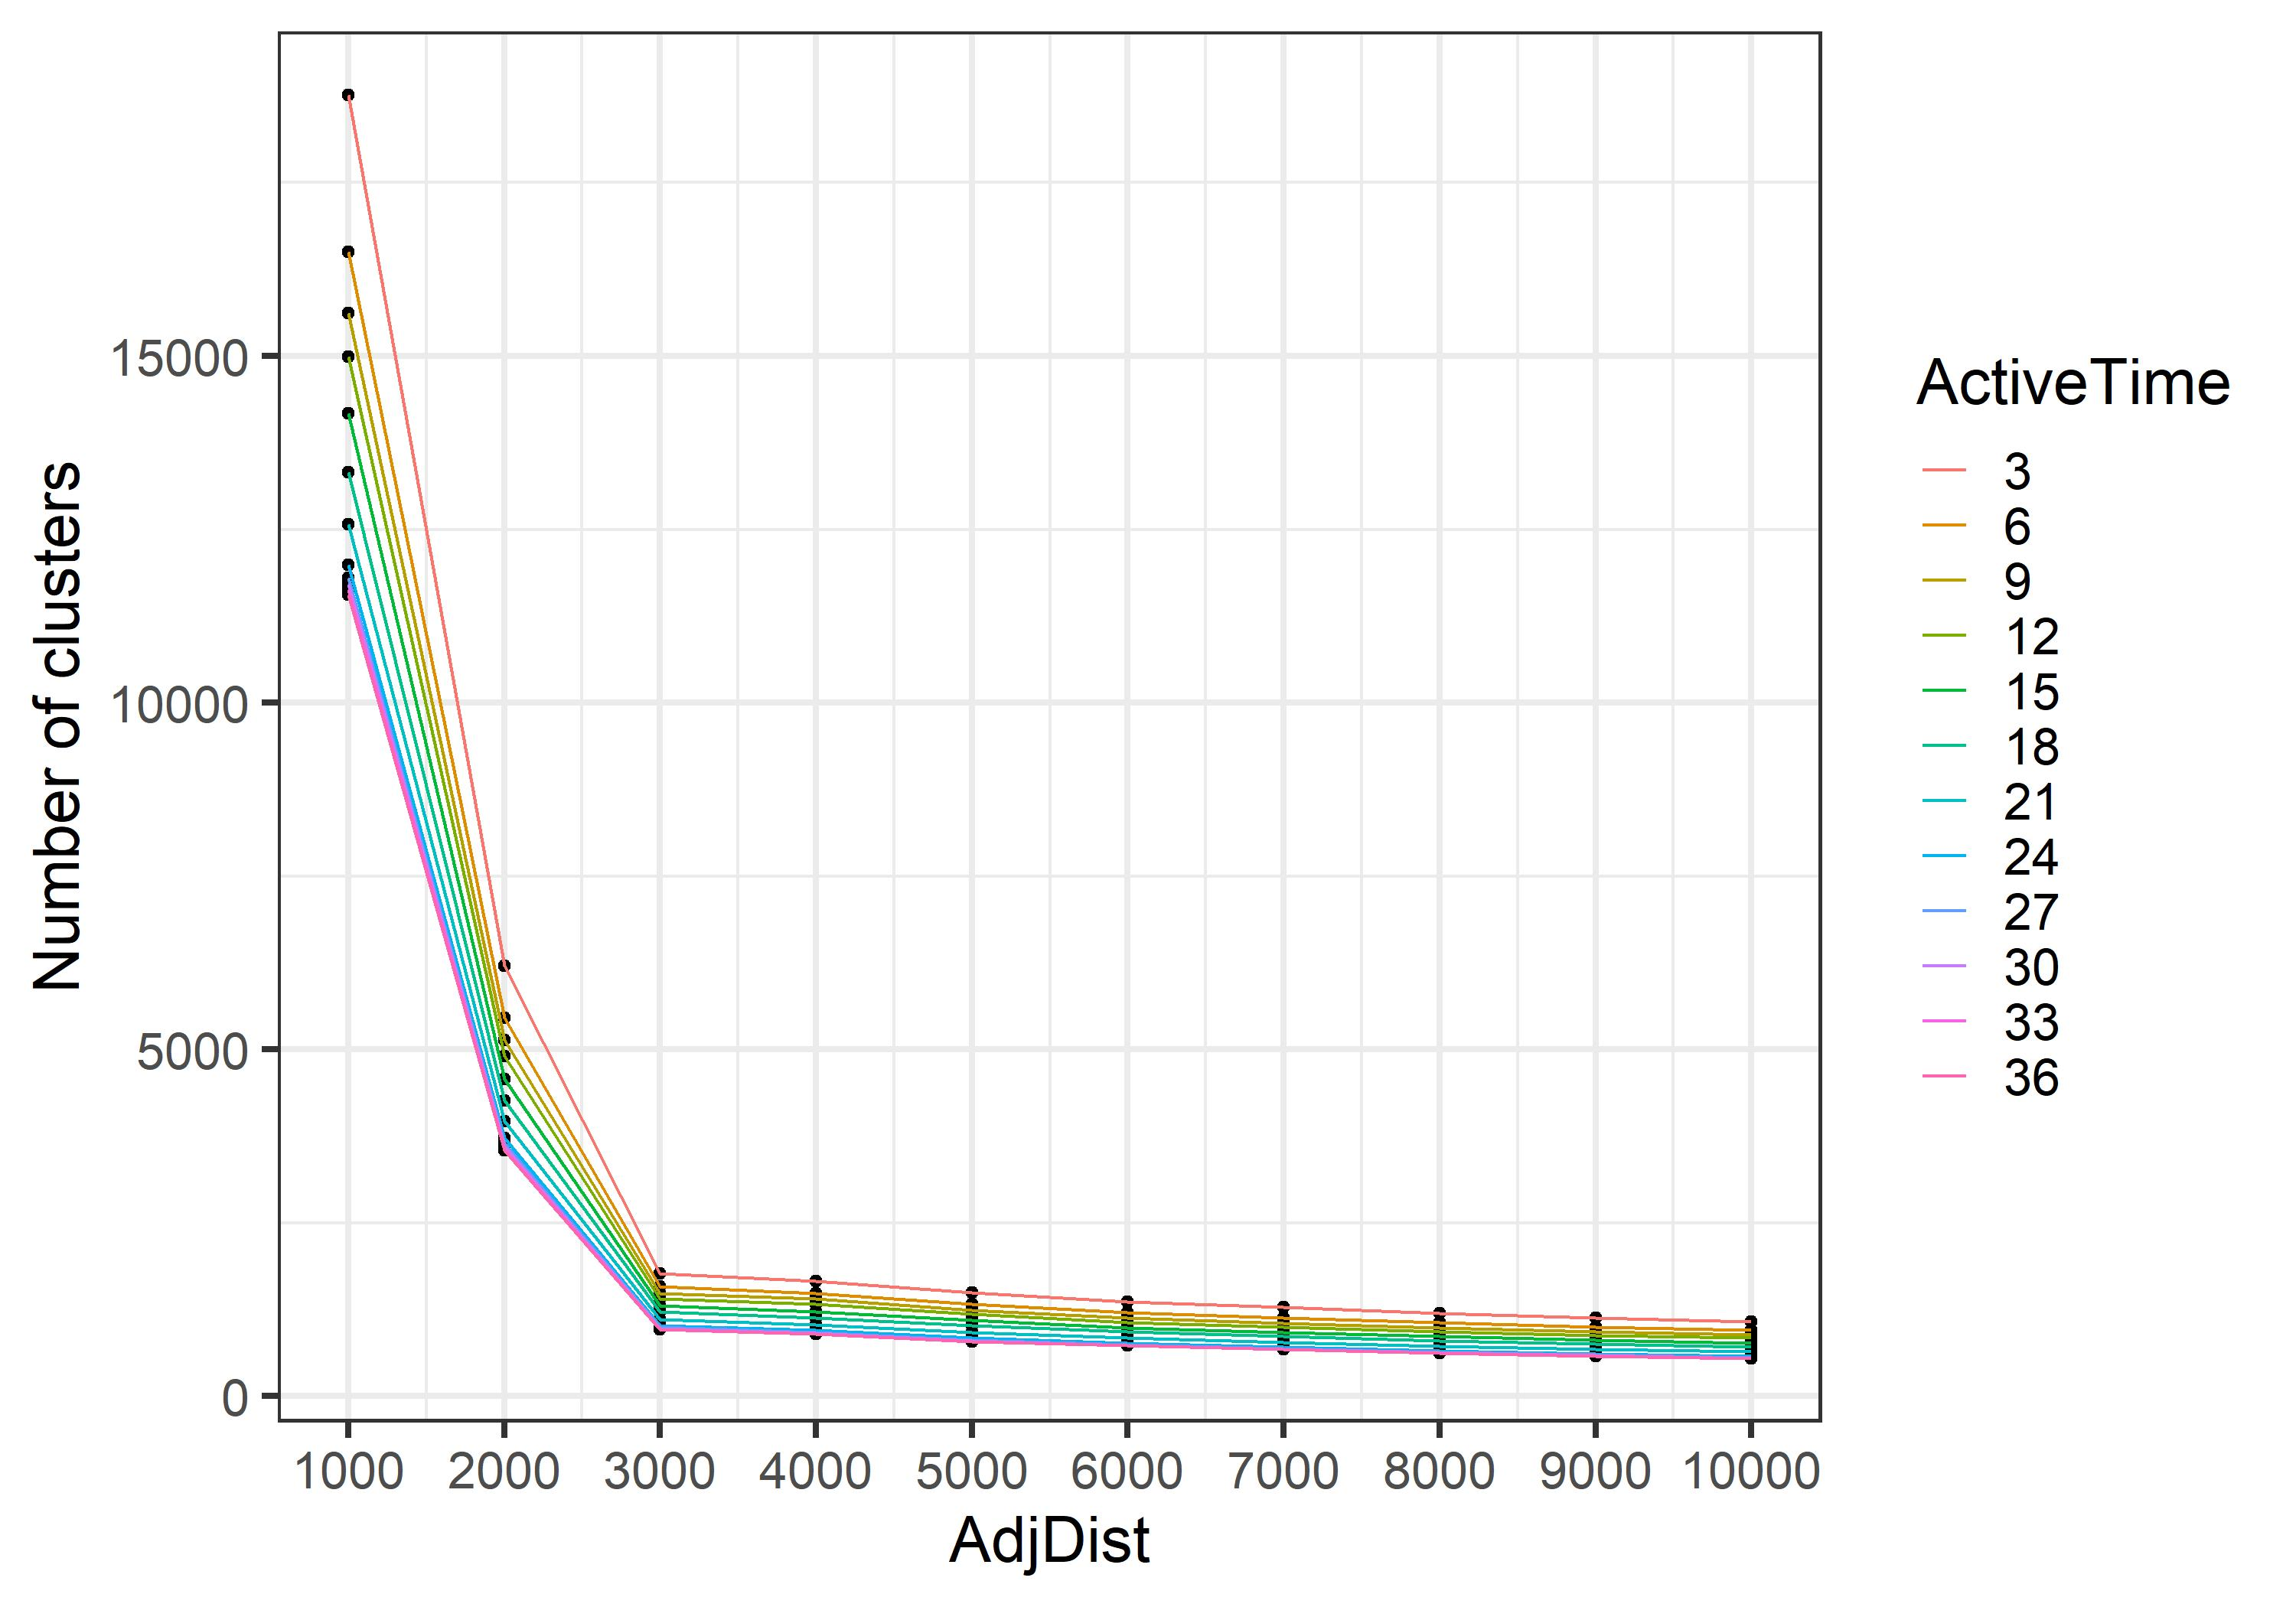
\includegraphics[width=0.8\linewidth]{figures/clustering_tuning_1} 

}

\caption[A visualization tool for parameter tuning ]{A visualization tool for parameter tuning . It works like a scree plot. Major falls of the number of clusters are observed when $AdjDist < 3000$ so the reasonable choice of $AdjDist$ is 3000m.}\label{fig:vis1}
\end{figure}
\end{Schunk}

\begin{Schunk}
\begin{figure}

{\centering 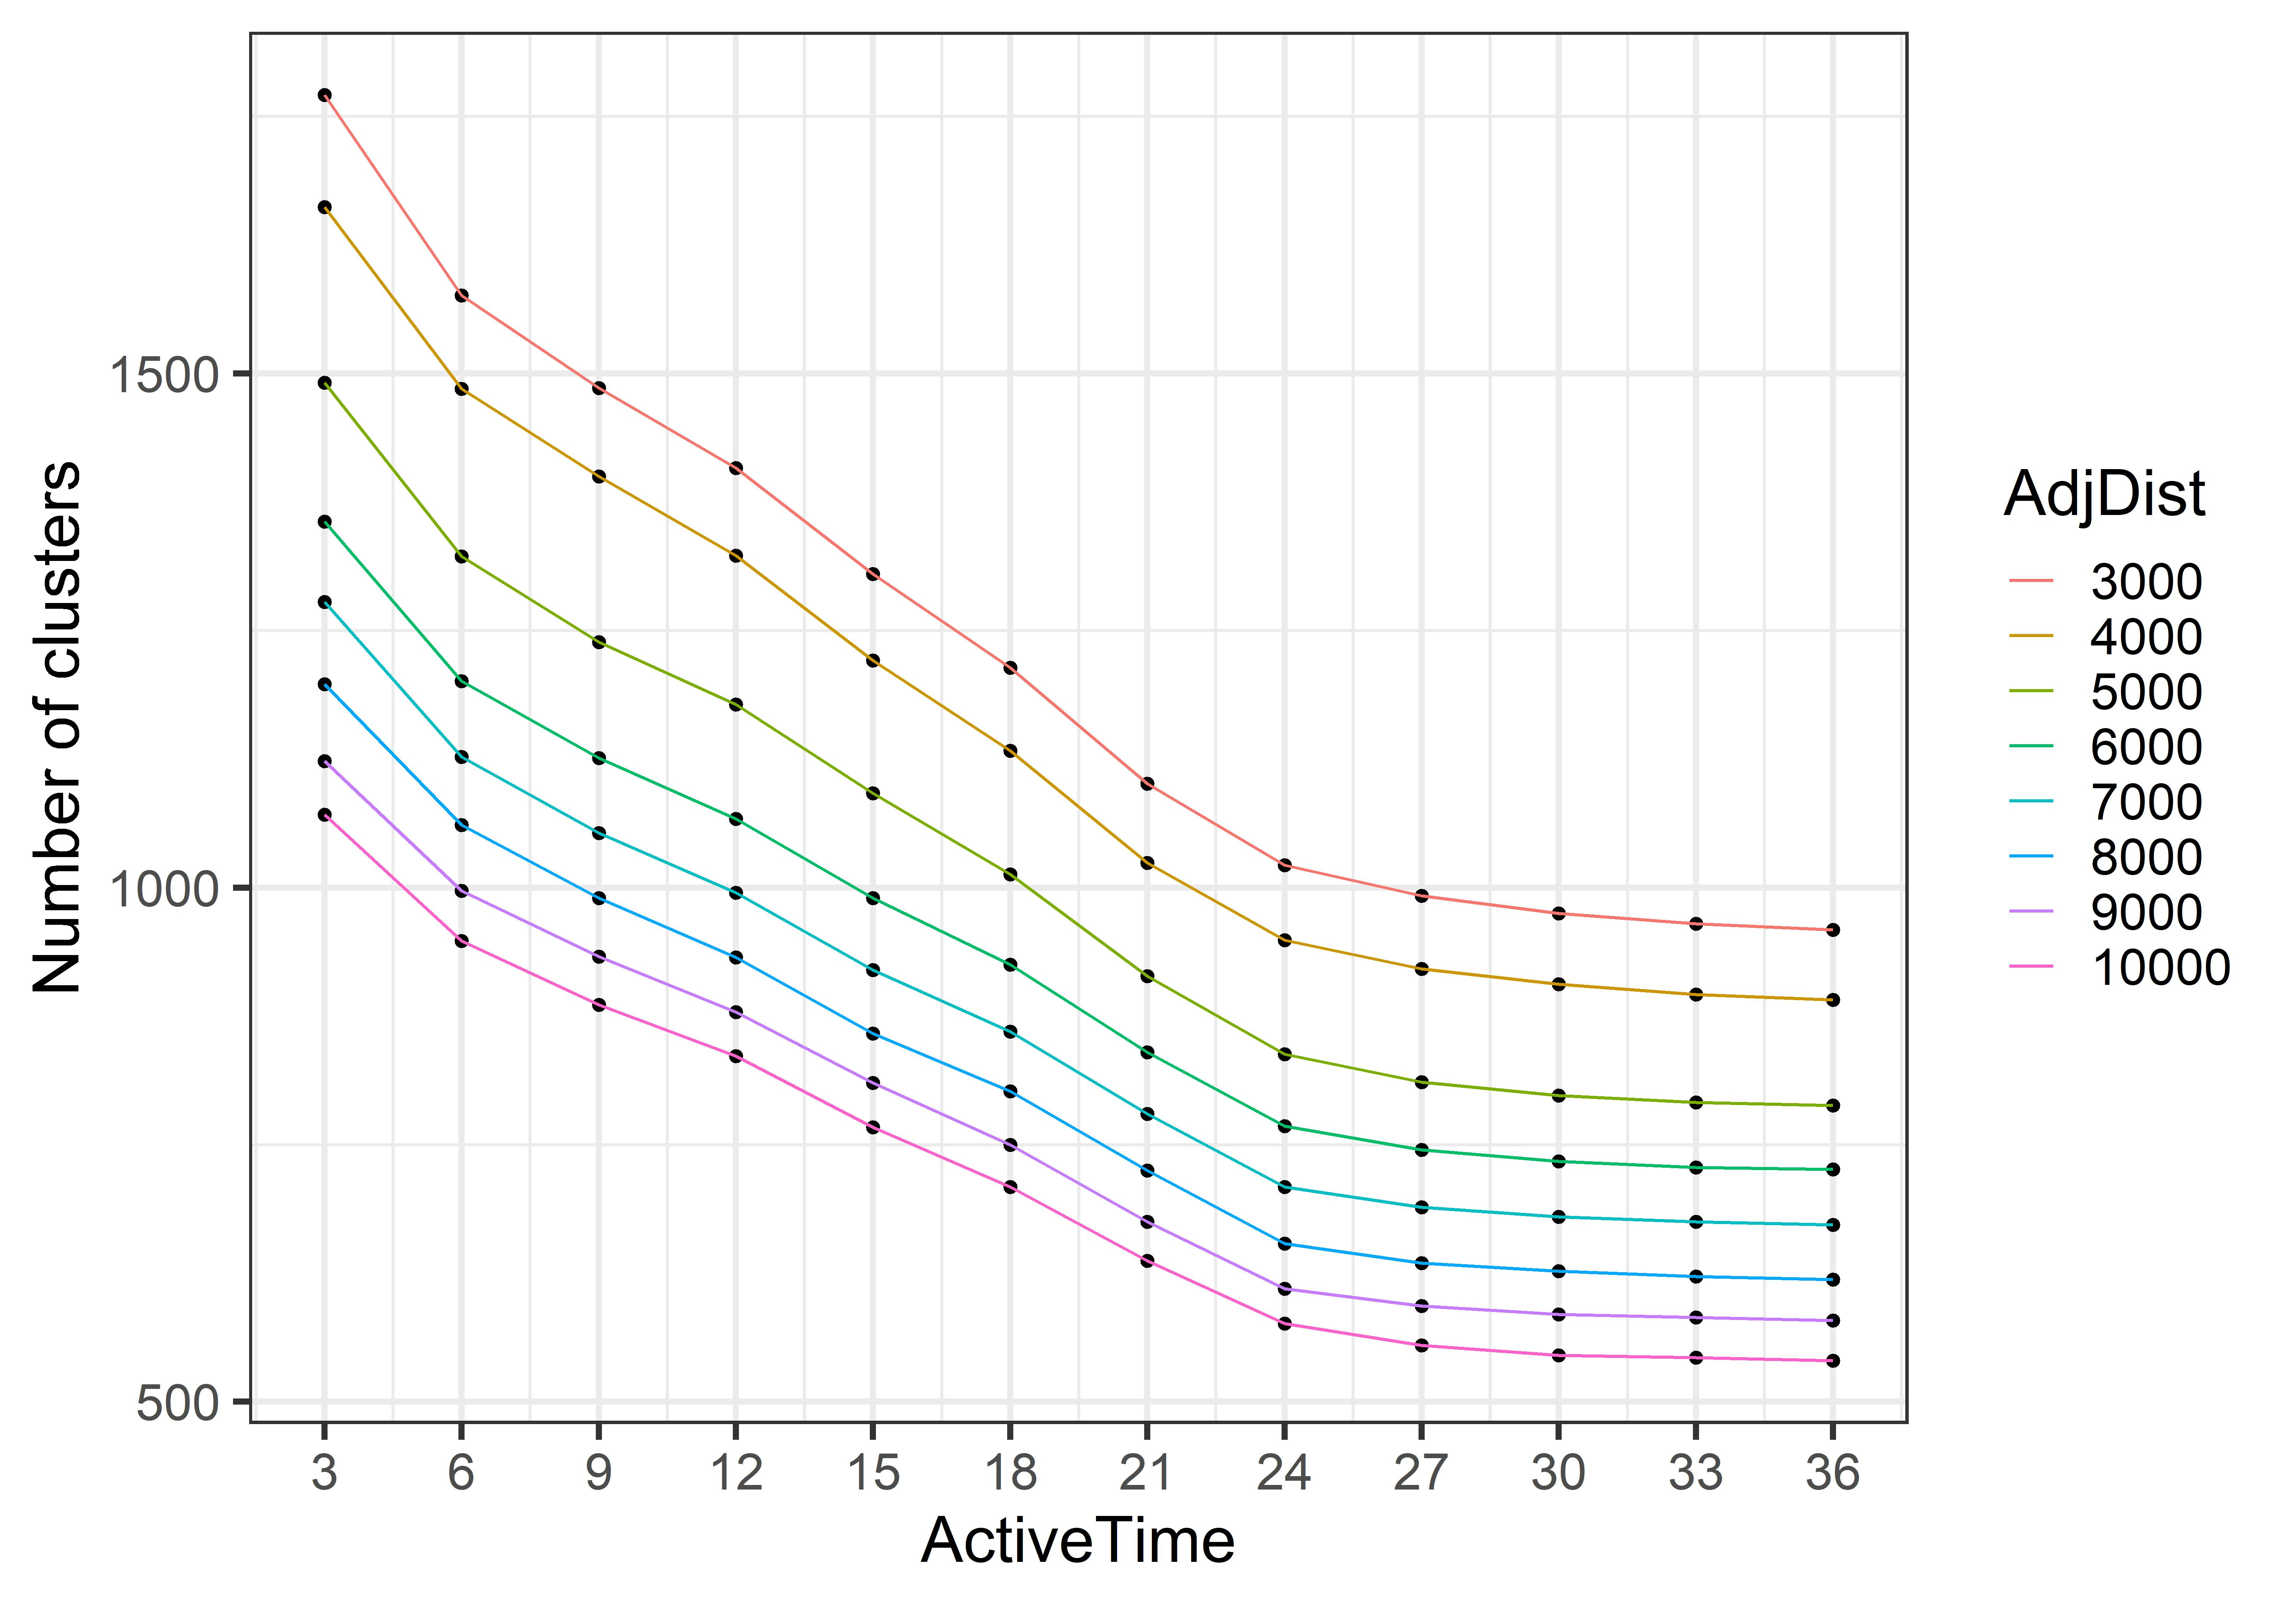
\includegraphics[width=0.8\linewidth]{figures/clustering_tuning_2} 

}

\caption[Major falls of the number of clusteres are observed when $ActiveTime < 24$, so the reasonable choice of $ActiveTime$ is 24 hours]{Major falls of the number of clusteres are observed when $ActiveTime < 24$, so the reasonable choice of $ActiveTime$ is 24 hours.}\label{fig:vis2}
\end{figure}
\end{Schunk}

\hypertarget{application}{%
\subsection{Application}\label{application}}

\hypertarget{determining-the-ignition-point-and-time-for-individual-fires}{%
\subsubsection{Determining the ignition point and time for individual
fires}\label{determining-the-ignition-point-and-time-for-individual-fires}}

Show ignition points for a particularly heavy day and another for a
particularly light day

\begin{Schunk}
\begin{figure}

{\centering 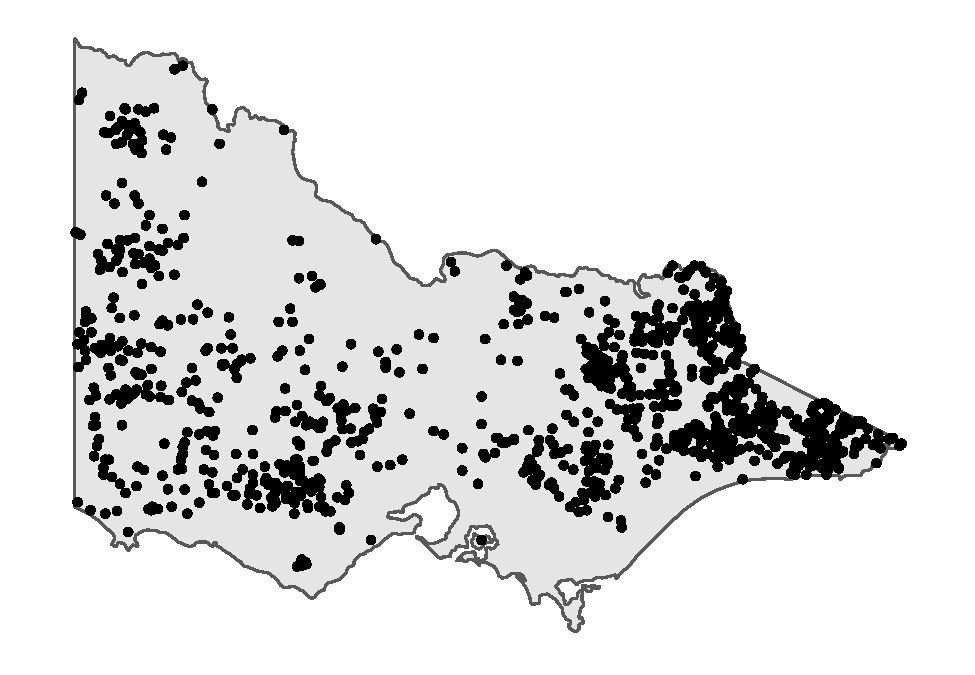
\includegraphics[width=0.8\linewidth]{clustering_paper_files/figure-latex/app1-1} 

}

\end{figure}
\end{Schunk}

\begin{Schunk}
\begin{figure}

{\centering 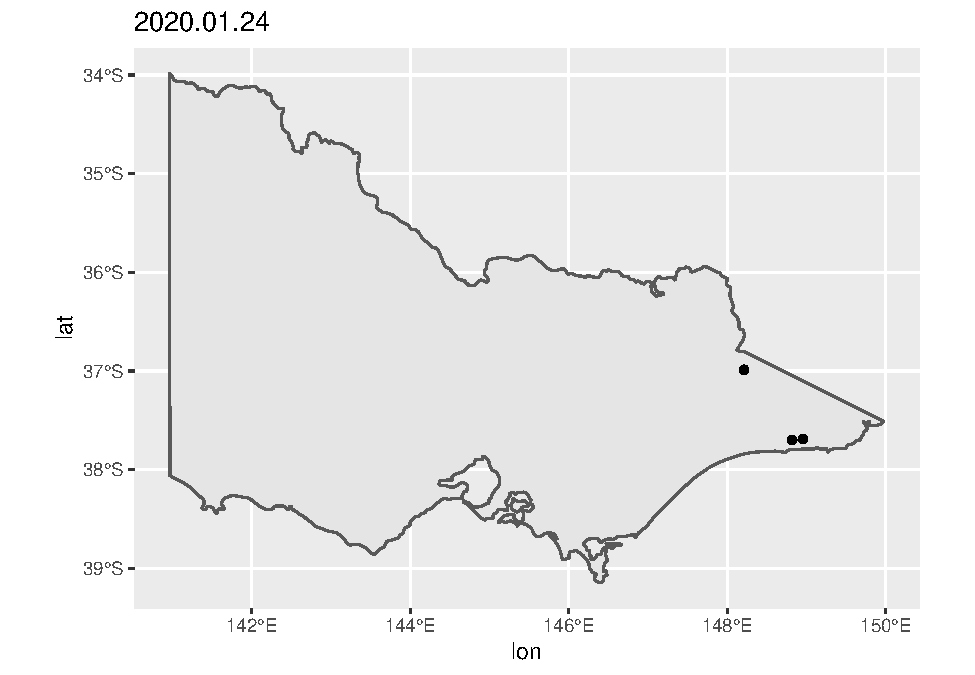
\includegraphics[width=0.8\linewidth]{clustering_paper_files/figure-latex/app2-1} 

}

\end{figure}
\end{Schunk}

\begin{Schunk}
\begin{figure}

{\centering 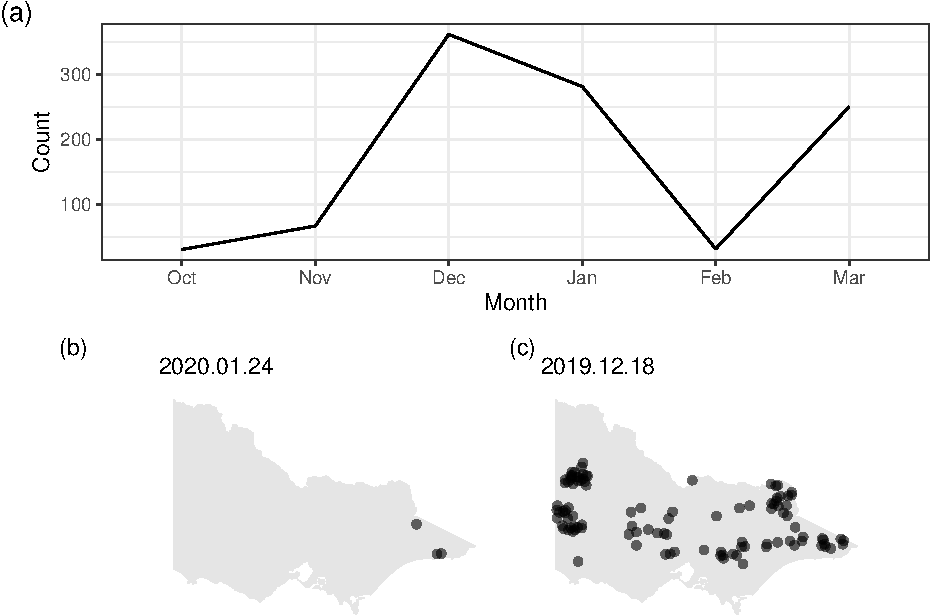
\includegraphics[width=0.8\linewidth]{clustering_paper_files/figure-latex/app3-1} 

}

\end{figure}
\end{Schunk}

\hypertarget{tracking-fire-movement}{%
\subsubsection{Tracking fire movement}\label{tracking-fire-movement}}

Display showing how a fire moves over time, maybe two or more fires

\hypertarget{allocating-resources-for-future-fire-prevention}{%
\subsubsection{Allocating resources for future fire
prevention}\label{allocating-resources-for-future-fire-prevention}}

Merging data with camp sites, CFA, roads, \ldots{}

\hypertarget{summary}{%
\subsection{Summary}\label{summary}}

\hypertarget{acknowledgements}{%
\subsection{Acknowledgements}\label{acknowledgements}}

\begin{itemize}
\tightlist
\item
  The code and files to reproduce this work are at XXX
\item
  Data on hotspots can be downloaded from XXX
\end{itemize}

\bibliography{RJreferences}


\address{%
Weihao Li\\
Monash University\\%
line 1\\ line 2\\
%
%
%
\\\href{mailto:wlii0039@student.monash.edu}{\nolinkurl{wlii0039@student.monash.edu}}
}

\address{%
Emily Dodwell\\
AT\&T\\%
line 1\\ line 2\\
%
%
%
\\\href{mailto:emdodwell@gmail.com}{\nolinkurl{emdodwell@gmail.com}}
}

\address{%
Dianne Cook\\
Monash University\\%
line 1\\ line 2\\
%
%
%
\\\href{mailto:dicook@monash.edu}{\nolinkurl{dicook@monash.edu}}
}

